\section{Introduction}

% What is the problem?
Migrating resources is a useful tool for optimizing performance for systems
that service highly accessed data\footnote{In this paper, we use the term
``data" to refer to the partitioned key-value pairs AND file system metadata.}
but deciding how to make the migrations is a risky trade-off. Data can be
distributed to alleviate overloaded servers or it can be concentrated to
exploit locality. These techniques are at odds and selecting the wrong technique
can have catastrophic consequences. For example, migrating data to an
already overloaded server or increasing the network hops by spreading data
across an underutilized cluster will impact performance negatively.

% Why is concentration vs. distribution difficult?
Unfortunately, deciding which optimization to use is difficult to reason about,
especially with the scale and complexity of today's HPC architectures. While
the mechanisms are usually built into the systems, the policies often times
less refined and much more sensitive to the workload. So a system may have the
ability exploit locality using techniques like bulk operations, multiple
partition strategies, secondary indexes, and caching but deciding when, where,
and how to use them is workload dependent and difficult to figure out.

% What we did in the paper
This paper takes an API designed to migrate file system metadata and applies it
to an HPC key-value store.  The API helps control distribution and
concentration by letting the administrator define how to migrate load, where to
migrate load, and how much load to migrate. While designed for a different
domains, this API encompasses many of the same properties we need for an HPC
key-value store, namely:

\begin{itemize}
  \item services small/frequent requests
  \item popularity drives distribution
  \item locality drives concentration
\end{itemize}

\begin{figure}[t]
  \noindent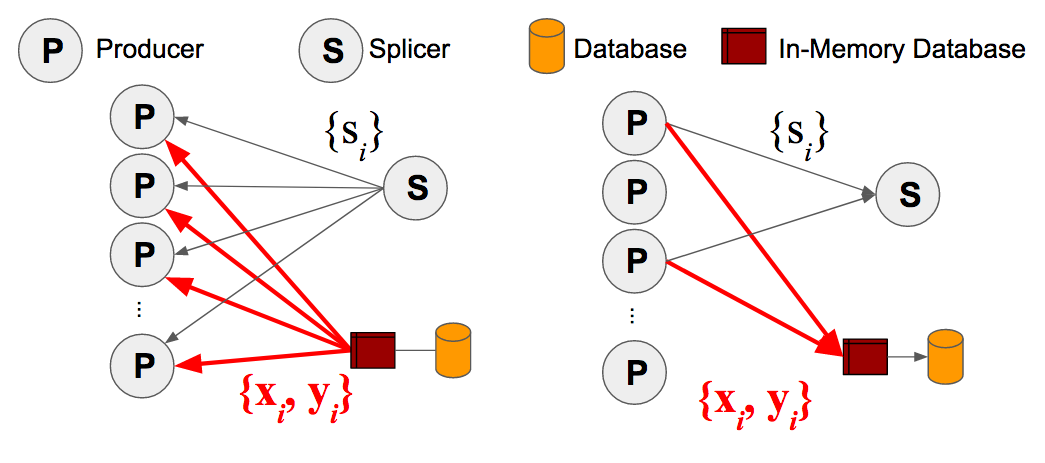
\includegraphics[width=19pc,angle=0]{figures/arch-parsplice.png}\\
  \caption{ParSplice is a ready-heavy HPC application where producers use a
  database for consistency. Replacing the single-node database with HXHIM
  improves performance with load balancing.
  \label{fig:arch-parsplice}}
\end{figure}

% Why is HXHIM a good fit?
To show the efficacy of this approach, we examine the ParSplice molecular
dynamics simulation application shown in Figure~\ref{fig:arch-parsplice}.
ParSplice uses a single-node database for consistency, where producers, \(P\),
push and pull coordinates, \{\(x_i, y_i\)\}, based on the segments,
\{\(s_i\)\}, assigned by the splicer, \(S\). In this paper, we replace the
database with a distributed key-value store designed for HPC enjoy performance
optimizations for:

\begin{itemize}
  \item \texttt{put()} because of the distributed sync and load balancing based on:
  \begin{itemize}
    \item lazy synchronization with tombstones and RPCs
    \item strong synchronization with consensus and blocking
  \end{itemize}
  \item \texttt{get()} because of the load balancing
\end{itemize}

It has 4 phases:

\begin{enumerate}

  \item splicer (S) tells producers (P) to compute segments for state \(s_i\)

  \item P's pull initial coordinates \{\(x_i, y_i\)\} from database

  \item a P inserts completed coordinates for segment \(s_i\) into database and
  S broadcasts next segment(s) \(s_j\) 

  \item P's pull new segment coordinates \{\(x_j, y_j\)\}
\end{enumerate}

, which has both a high computational footprint and data locality.
The former suggests distribution to avoid hot spots while the latter encourages
concentration to leverage the database's secondary indeices, bulk operations,
and key redistribution functionality. 

% Why is HXHIM a good fit?
To show this approach at scale we study
ParSplice~\cite{perez:jctc20150parsplice}, an HPC dynamics simulator that has
both a high computation footprint, which suggests distribution to avoid hot
spots, and data locality, which alternatively encourages concentration so the
key-value store can use its functionality for secondary indices, bulk
operations, and key redistribution. ParSplice uses both molecular dynamic (MD)
and accelerated molecular dynamic methods (AMD) for simulations with long
periods of inactivity and short periods of ``interesting" events.  Molecules in
periods with many events are simulated with MD methods, which are exact but can
only be run for a fixed, short period of time because the cumulative error
grows so large. Alternatively, longer trajectories are simulated with AMD
methods, which use statistics and parallelization to show the less precise
state-to-tate trajectories. ParSplice tackles ``low-barrier problems", where
the types of energy barriers separating states of the system are non-uniform
(i.e. some require less energy than others). It chops long trajectories into
parallelizable units called segments, where the segments can also be spliced
together to form longer trajectories; this approach allows ParSplice to trade
off accuracy for speed in a configurable way.

% How is ParSplice implemented?
ParSplice stores segments in a database while it runs. The splicer pastes
segments generated by \(n\) producers.

% What do we contribute?
In this paper, we make the following contributions:

\begin{enumerate}

  \item protype that controls concentration and distribution using the bulk
  operations, secondary indicies, and cursor types mechanisms
  from~\cite{greenberg:hotstorage2015-mdhim}. 

  \item quantifies benefits of server/client-side caching, many small messages,
  and bulk operations.

\end{enumerate}
